\documentclass{article}
\usepackage{iclr2027_conference,times}

\input{math_commands.tex}

\usepackage{graphicx}
\usepackage{caption}
\usepackage{subcaption}
\usepackage{booktabs}
\usepackage{multirow}
\usepackage{array}
\usepackage{makecell}
\usepackage{siunitx}
\sisetup{
  group-separator={,},
  group-minimum-digits=4,
  table-number-alignment=center,
  detect-weight=true,
  detect-inline-weight=math,
}
\usepackage{microtype}
\usepackage{hyperref}
\usepackage{url}

% Floats may share pages with body text above and below (table + figure in §2.2).
\setcounter{topnumber}{2}
\setcounter{bottomnumber}{2}
\setcounter{totalnumber}{4}
\renewcommand{\bottomfraction}{0.65}
\renewcommand{\floatpagefraction}{0.85}

\title{Charts as Epistemic Actions: Experience-Driven Multimodal Analysis in Data Agents}

% Keep the submission anonymous. Do not uncomment \iclrfinalcopy.
\author{Anonymous Authors}

\newcommand{\method}{\textsc{CARE}}
\newcommand{\probe}{\textsc{ProbeTask}}
\newcommand{\na}{\textemdash}
\newcommand{\headpct}{(\%)}
\newcommand{\tabpubliclyreported}[1]{%
  \multicolumn{#1}{l}{\textit{Publicly reported benchmark scores}}\\%
}
\newcommand{\placeholderfigure}[2]{%
  \fbox{\begin{minipage}[c][#1][c]{0.94\linewidth}
    \centering\small\textbf{#2}\\[0.5em]
    Final source figure not yet available.
  \end{minipage}}}

\begin{document}

\maketitle

\begin{abstract}

  % 图表是人类分析师识别趋势、模式和异常的重要认知工具。尽管多模态大语言模型（MLLM）能够解读图表，但图表对于数据分析智能体的分析效用仍缺乏深入研究。在本文中，我们首先基于标注问题设计了一项探究实验，考察模型解读图表证据的能力，及其在开放式自主分析中的图表使用行为我们发现，受评测模型能有效的从图和表中提取有效分析证据，但在自主分析中是否主动使用chart方面存在显著的模型差异。此外，图表与文本呈现出任务依赖的能力互补性。上述结果表明，图表不应仅被视为事后呈现工具，而应成为数据分析智能体推理过程的内在组成部分。基于这一认识，我们进一步提出 CARE，通过比较采用不同证据表征的分析轨迹，协同演化分析经验与表征经验，帮助智能体学习如何构建、选择和使用图表证据，并缓解其模态使用偏置。在四个基准上的实验表明，CARE能够促进模型主动利用图表开展分析，并显著优于基线方法。
  
  Charts are important cognitive tools that help human analysts identify trends, patterns, and anomalies. Although multimodal large language models (MLLMs) can interpret charts, the analytical utility of charts for data-analysis agents remains underexplored. In this work, we first conduct a probe study based on annotated questions to examine models' ability to interpret evidence from charts and their chart-use behavior in open-ended autonomous analysis. We find that the evaluated models effectively extract useful evidence from charts and tables, but differ substantially in whether they actively use charts during autonomous analysis. Moreover, charts and text exhibit task-dependent complementarity. These findings suggest that charts should not serve merely as post-hoc presentation tools, but should form an intrinsic part of data-analysis agents' reasoning. Building on this insight, we propose \textbf{C}o-evolving \textbf{A}nalysis and \textbf{R}epresentation \textbf{E}xperiences. \textsc{CARE} contrasts analysis trajectories with different evidential representations to jointly evolve analytical and representational experience. This approach helps agents learn how to construct, select, and use chart-based evidence while mitigating modality-use biases. Experiments on three held-out benchmarks show that \textsc{CARE} encourages models to actively use charts for analysis and significantly outperforms baseline methods.
\end{abstract}

\section{Introduction}
\label{sec:introduction}

Data agents are intelligent systems centered on large language models (LLMs) that interpret analytical goals, access data environments, invoke analytical tools, and produce data-grounded insights.
Recent progress in ReAct-style reasoning--acting loops and tool use~\citep{yao2023react} has strengthened autonomous planning, code execution, and iterative analysis, moving data agents from proof-of-concept demonstrations toward practical assistants capable of complex tasks---a promising path for business decision-making, scientific inquiry, and data-science automation.

Nevertheless, most data agents still conduct analysis primarily in text.
Models generate Text-to-SQL queries or Python scripts from a schema and advance reasoning from textualized execution results.
Human analysts rely on charts to recognize trends, distributions, anomalies, and relationships among variables; they externalize candidate patterns visually and then select further computation and verification accordingly.
Why has this step not yet been fully integrated into the data-agent analytical loop?
More generally, \emph{in what form should intermediate analytical evidence and insights be presented so that information is preserved and subsequent reasoning is supported?}
The question concerns not only whether to use charts, but also how analytical results should be organized, represented, and consumed.

Prior work on charts follows three broad lines: generation, understanding, and representation selection.
Generation methods produce and refine visualizations from data and user intent, improving data fidelity and chart quality~\citep{dibia2023lida,yang2024matplotagent,yang2025chartmimic,namgoong2025amace,lu2026multivisagent,wang2025chartoptimiser}.
Understanding methods strengthen interpretation through structure recovery, numerical reasoning, and visual tools~\citep{masry2023unichart,han2023chartllama,xu2023chartbench,liu2023deplot,liu2023matcha,zhang2024tinychart,kaur2026chartagent,das2025chartsofthought}.
Multimodal representation research compares textual and visual encodings of the same information and shows that representation choice affects reasoning outcomes~\citep{zhou2025fres,ho2026formatmatters,xing2026tabledart,lin2026evidfuse}.
These strands typically target specified chart generation, interpretation of externally supplied charts, or selection among preset representations.
They have not systematically measured the benefit of charts in \emph{open-ended} data analysis, nor answered whether data agents can productively exploit open plotting capabilities or which kinds of analytical evidence charts versus text should carry.

To assess the practical utility of charts for data agents, we construct \probe{} from synthetic analysis trajectories and examine chart-reading competence, behavior under open plotting tools, and the performance of charts and text across analytical tasks and cognitive demands.
Two main findings emerge.
First, evaluated models can extract useful evidence from charts, yet they do not reliably convert access to plotting tools into consistent analytical gains---a pronounced \emph{capability--utility} gap.
Second, charts and text serve as task-dependent, complementary evidence representations: charts are better suited to trends, patterns, and anomalies, whereas text excels at precise reading, conditional verification, and integrating multiple pieces of evidence.
These results indicate that how intermediate evidence is represented directly shapes analytical reasoning; because utility varies with task and analytical stage, representation strategy should be learned from trajectories and outcome feedback rather than reduced to fixed task-to-modality rules.

Motivated by this view, we propose \method{} (\textbf{C}o-evolving \textbf{A}nalysis and \textbf{R}epresentation \textbf{E}xperiences), which jointly evolves analytical and representational experience.
For each task, \method{} samples multiple analysis trajectories and compares their final outcomes to distill two kinds of reusable knowledge: what analytical evidence to construct, and how to present and use that evidence.
The two experience types are stored in separate repositories but updated and version-selected jointly according to task performance under their combined effect.
At inference time, the data agent retrieves relevant experiences given the current task, analytical operation, and intermediate results, and dynamically decides subsequent analysis steps and whether to use text, charts, or a hybrid---without hand-crafted modality-routing rules.
We evaluate \method{} on several external data-analysis benchmarks held out from experience evolution, and use ablations with single experience types, chart disabling, and non-evolved experience to test the incremental value of dual-experience co-evolution and visual representation.

In summary, our main contributions are as follows:
\begin{itemize}
  \item We systematically probe the analytical utility of charts for data agents on synthetic trajectories (\probe{}), revealing a gap between chart understanding and productive use of open plotting, and summarizing task-dependent complementarity between charts and text as evidence representations.
  \item We propose \textsc{CARE} (Co-evolving Analysis and Representation Experiences), which jointly evolves analytical and representational experience from outcome-scored trajectories so that agents learn both what evidence to construct and how to represent and use it, without hand-crafted modality-routing rules.
  \item Experiments on three external data-analysis benchmarks (DDR-Bench, DAComp-DA, and DSBench) with six LLM backbones demonstrate that \textsc{CARE} consistently outperforms matched baseline agents; ablations on single experience types, chart disabling, and non-evolving experience quantify the contribution of dual-experience co-evolution and visual representation.
\end{itemize}



\section{Charts in the Analytical Loop}
\label{sec:probe}

In this section, we construct \probe{} from synthetic analysis trajectories and evaluate data agents in a realistic tool-use loop with open plotting.
We first describe the task suite, metrics, and agent settings (\S\ref{sec:probe-setup}), then analyze chart-reading competence, autonomous modality use, and the complementary roles of text and charts (\S\ref{sec:probe-findings}).

\subsection{Exploratory Probe Design}
\label{sec:probe-setup}

\paragraph{Probe construction.}
Our goal is to isolate how representations of intermediate results affect analytical reasoning, rather than to introduce another end-to-end data-analysis benchmark.
This requires tasks that pair raw tables and open-ended questions with executable analyses and reference insights.
InsightBench~\citep{sahu2025insightbench} provides these elements over enterprise tables and therefore supports controlled interventions on the agent's analytical interface.
We take its first 50 source-data flags and split each associated insight unit into one ProbTask.
This process yields 219 candidates.
After excluding 17 tasks with empty questions, we retain 202 evaluable tasks from 49 flags.

Each ProbTask contains a raw CSV table, a dataset description, an analytical question, a reference analysis, and a target insight.
The agent receives the table and question, together with the description, schema, and first three rows as initial context.
The target insight remains hidden and is used only for evaluation.
The agent must select and execute the required operations, such as filtering, feature derivation, aggregation, sorting, temporal transformation, or statistical testing, and return a direct natural-language answer.

\paragraph{Task annotation.}
We use two complementary taxonomies for post-hoc analysis.
\emph{Question type} specifies the answer sought by a task: numeric lookup, composition, rank or extreme, group comparison, temporal change, relationship, anomaly or risk, diagnosis, or prediction.
\emph{Cognitive load} specifies the primary operation required to derive the answer from an intermediate analytical view: locate, scan and select, compare, recognize a pattern, interpret a relation, integrate dimensions, or perform conditional reasoning.
An LLM first assigns each label from the task evidence, after which a human annotator reviews and confirms it.
The resulting labels support only post-hoc slice analysis; they never define hand-crafted modality-routing rules.

\paragraph{Metrics.}
A common GPT-5.6 Sol judge scores each answer against the question and target insight on a 0--4 scale.
We map normalized judge scores to $[0,100]$ and report their mean.
Slice analyses use task-paired differences with flag-clustered bootstrap intervals~\citep{efron1993bootstrap} and randomization tests.

\paragraph{Agent settings.}
All settings share the same vanilla ReAct agent with one general-purpose Bash tool.
Each call starts a fresh process, while files persist in a shared working directory and the CSV is exposed read-only.
We hold the task, model, initial context, interaction limit, and tool budget fixed across groups; only the analytical interface differs:
\begin{itemize}
  \item \textbf{No-tool:} no execution tool; the agent answers from the description, schema, and three example rows only.
  \item \textbf{Text-only:} tool output exposes stdout and stderr; plotting is prohibited.
  \item \textbf{Chart-only:} stdout is hidden; the agent receives generated pixel images and stderr, with analytical results explicitly prohibited in stderr.
  \item \textbf{Free-style:} stdout, stderr, and pixel images are all returned; the agent may use text, charts, or both.
\end{itemize}

\noindent\textbf{Experiments.}
On the full \probe{} suite ($n{=}202$), we run an \emph{interface ablation} with GPT-5.6 Sol under all four settings above, and a separate \emph{model comparison} with six backbones---Claude Opus 5, Claude Sonnet 5, GPT-5.6 Luna, GPT-5.6 Sol, DeepSeek V4.1 Flash, and HY3---under the Free-style interface.
The same GPT-5.6 Sol judge scores every run.
In \S\ref{sec:probe-findings}, we analyze these results in depth.


\begin{table}[t]
	\centering
	\hfill
	\begin{minipage}[t]{0.32\textwidth}
		\centering
		\small
		\captionof{table}{Interface ablation on \probe{} with gpt-5.6-sol: scores for each of the four agent settings.}
		\label{tab:four-condition}
		\vspace{0.35em}
		\begin{tabular}{@{}lr@{}}
			\toprule
			Agent configuration & Score \\
			\midrule
			No-tool & 29.4 \\
			Text-only & 77.2 \\
			Chart-only & 78.4 \\
			Free-style & 77.6 \\
			\bottomrule
		\end{tabular}
	\end{minipage}\hfill
	\begin{minipage}[t]{0.62\textwidth}
		\centering
		\captionof{table}{Free-style on \probe{} across six LLM backbones: score; modality use (\# tasks); mean ReAct rounds and tokens.}
		\label{tab:model-bias}
		\vspace{0.35em}
		{\setlength{\tabcolsep}{4pt}%
			\renewcommand{\arraystretch}{1.12}%
			\newcolumntype{M}{>{\centering\arraybackslash}p{1.85em}}%
			\scriptsize
			\begin{tabular}{@{}l@{\hspace{1em}}c@{\hspace{1em}}c@{\hspace{1.5em}}c@{\hspace{0.5em}}c@{\hspace{0.5em}}c@{\hspace{1em}}c@{}}
				\toprule
				\multirow{2}{*}[-0.15em]{LLM backbone} &
				\multirow{2}{*}[-0.15em]{Score} &
				\multicolumn{3}{c}{Used modality (\# tasks)} &
				\multicolumn{2}{c}{ReAct cost} \\
				\cmidrule(lr){3-5}%
				\cmidrule(lr){6-7}
				& & Text & Chart & Both & Rounds & Tokens \\
				\midrule
				Claude Opus 5 & 83.1 & 43 & 0 & 157 & 3.9 & 17{,}401 \\
				Claude Sonnet 5 & 79.2 & 102 & 0 & 98 & 4.0 & 18{,}724 \\
				GPT-5.6 Luna & 76.2 & 198 & 0 & 2 & 3.1 & 6{,}835 \\
				GPT-5.6 Sol & 77.6 & 198 & 0 & 2 & 2.9 & 6{,}392 \\
				DeepSeek V4.1 Flash & 80.2 & 143 & 0 & 57 & 6.2 & 30{,}051 \\
				HY3 & 73.1 & 198 & 0 & 2 & 3.8 & 7{,}725 \\
				\bottomrule
		\end{tabular}}
	\end{minipage}\hfill
\end{table}

\subsection{Analysis and Findings}
\label{sec:probe-findings}

We now analyze the probe runs and summarize three sets of results: aggregate interface effects, model-specific modality use under Free-style, and slice-level complementarity between text and charts.

\paragraph{LLMs can conduct analysis through charts.}
Table~\ref{tab:four-condition} reports mean scores for the four agent settings.
GPT-5.6 Sol scores only 29.4 without tools, whereas its scores increase to 77.2 with text and 78.4 with charts. The chart condition therefore achieves performance comparable to the text condition and improves over the no-tool condition by 49.0 points. These results show that multimodal LLMs can extract sufficient analytical evidence from charts to answer data-analysis questions.

\paragraph{Open-ended modality choice exhibits strong model-specific bias.}
Table~\ref{tab:model-bias} compares Free-style trajectories across six LLMs, including modality-use patterns and interaction cost.
Marked variation appears under the same interface. Claude Opus 5 combines text and charts on 157 tasks, while Claude Sonnet 5 and DeepSeek V4.1 Flash do so on 98 and 57 tasks, respectively. In contrast, GPT-5.6 Luna, GPT-5.6 Sol, and HY3 use both modalities on only 2 tasks each and rely on text alone on the remaining 198. Chart-use frequency also has no monotonic relationship with performance: DeepSeek V4.1 Flash uses charts less often than Claude Sonnet 5 but attains a higher score, while the three low-frequency models obtain different scores despite identical use counts. Thus, access to the same multimodal interface does not produce a common modality-selection strategy; open-ended modality choice remains strongly shaped by model-specific priors.


\begin{figure}[t]
  \centering
  \captionsetup[subfigure]{skip=2pt}
  \begin{subfigure}[t]{\linewidth}
    \centering
    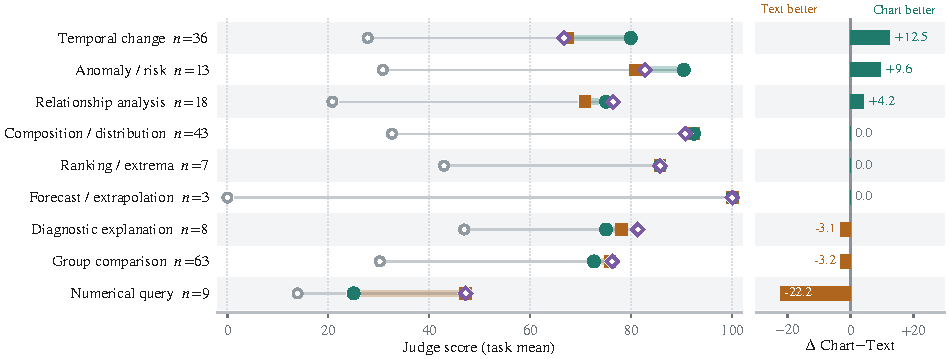
\includegraphics[width=\linewidth]{figures/probe_slices_dotplot_v3_a.pdf}
    \caption{Judge scores by question type.}
    \label{fig:probe-slices-a}
  \end{subfigure}
  \par\vspace{0.1em}
  \begin{subfigure}[t]{\linewidth}
    \centering
    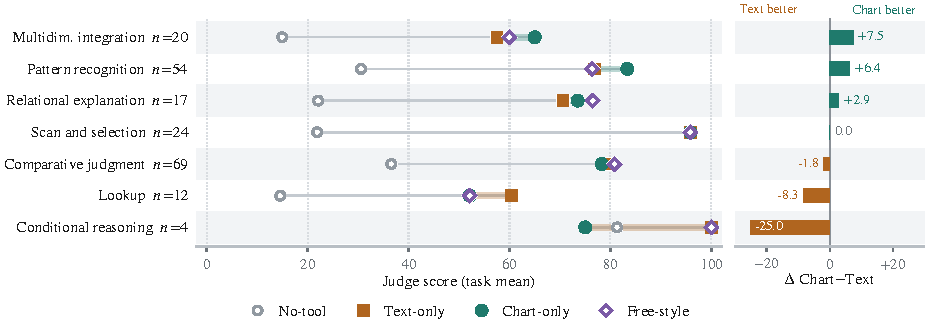
\includegraphics[width=\linewidth]{figures/probe_slices_dotplot_v3_b.pdf}
    \caption{Judge scores by primary cognitive load.}
    \label{fig:probe-slices-b}
  \end{subfigure}
  \caption{Slice analysis of the four agent settings on \probe{} ($n{=}202$).
    Markers show slice means; the right column gives Chart$-$Text $\Delta$ (faded when $n<10$).
    The bottom row of~\subref{fig:probe-slices-a} aggregates all tasks.}
  \label{fig:probe-slices}
\end{figure}

\paragraph{The advantage of charts is concentrated in change and pattern recognition.}
Figure~\ref{fig:probe-slices} breaks down the four settings by question type and cognitive load.
Charts score 0.799 on temporal-change questions, compared with 0.674 for text, yielding a gain of 0.125. Charts also lead by 0.096 on anomaly/risk questions and by 0.042 on relationship-analysis questions. The cognitive-load results exhibit the same pattern: charts score 0.833 on pattern recognition, exceeding text by 0.064, and lead by 0.029 on relational explanation and by 0.075 on multidimensional integration. In contrast, the two modalities perform similarly on composition/distribution, ranking/extrema, and scan-and-selection tasks. Free-style performs below the chart condition on both temporal change and pattern recognition, indicating that access to both modalities does not automatically preserve the advantages of visual representation.

\paragraph{Text is better suited to exact reading and conditional verification.}
Figure~\ref{fig:probe-slices} shows that text scores 0.472 on numerical queries, compared with 0.250 for charts, and scores 0.604 on lookup tasks, compared with 0.521 for charts. Text also has smaller advantages of 0.032 on group comparison and 0.018 on comparative judgment. On conditional reasoning, text scores 1.000 while charts score 0.750, although this slice contains only four tasks and therefore provides only exploratory evidence. Overall, the relative advantage of text is concentrated in tasks that require exact reading, information location, and conditional verification rather than in data-analysis tasks generally.

Taken together, these results reveal a gap between multimodal capability and effective multimodal analysis. Although current LLMs can extract useful evidence from self-generated charts, merely providing plotting tools does not ensure that agents will use them when beneficial or coordinate them with textual evidence. Their behavior remains strongly shaped by model-specific modality preferences, while the relative utility of text and charts varies across analytical demands. The central limitation is therefore not chart understanding alone, but the absence of a mechanism that jointly determines what analytical view to construct and how that view should be represented and used. Because these decisions depend on the task and the evolving analysis state, they cannot be reduced to a fixed task-to-modality routing rule. This motivates learning coupled analysis and representation strategies from completed trajectories and outcome feedback, as developed in the next section.


\section{\method{}: Co-Evolving Analysis and Representation Experiences}
\label{sec:care}

In this section, we present the \method{} framework.
We first describe the Dual Experience Library and its coupled analysis and representation experiences (\S\ref{sec:del}), then introduce how they are learned from outcome-guided trajectory comparison (\S\ref{sec:experience-learning}), and finally explain how they augment online data analysis (\S\ref{sec:online}).

Building on these findings, \method{} learns two coupled forms of conditional knowledge---analysis experience and representation experience---from outcome-scored trajectories.


\subsection{Dual Experience Library}
\label{sec:del}

The Dual Experience Library (DEL), $E=(E_A,E_R)$, stores two complementary forms of experience.
The analysis library $E_A$ recommends how to construct evidence, including operations, fields, filters, aggregation, ordering, and stopping criteria.
The representation library $E_R$ recommends how to present and consume the resulting view using text, charts, or both.
Each entry also records its applicable context, known failure modes, and provenance.

We separate the libraries because evidence construction and evidence consumption cause different failures and require different retrieval conditions.
Nevertheless, they are learned and applied jointly: analytical operations determine the available views, while representations affect which patterns are detected and which operations follow.
For example, $E_A$ may construct entity-level time series at a common temporal grain, and $E_R$ may use a shared-axis chart to identify trends followed by text to verify exact values.
Thus, \method{} uses \emph{decoupled storage but coordinated decisions}.


\begin{figure}[t]
  \centering
  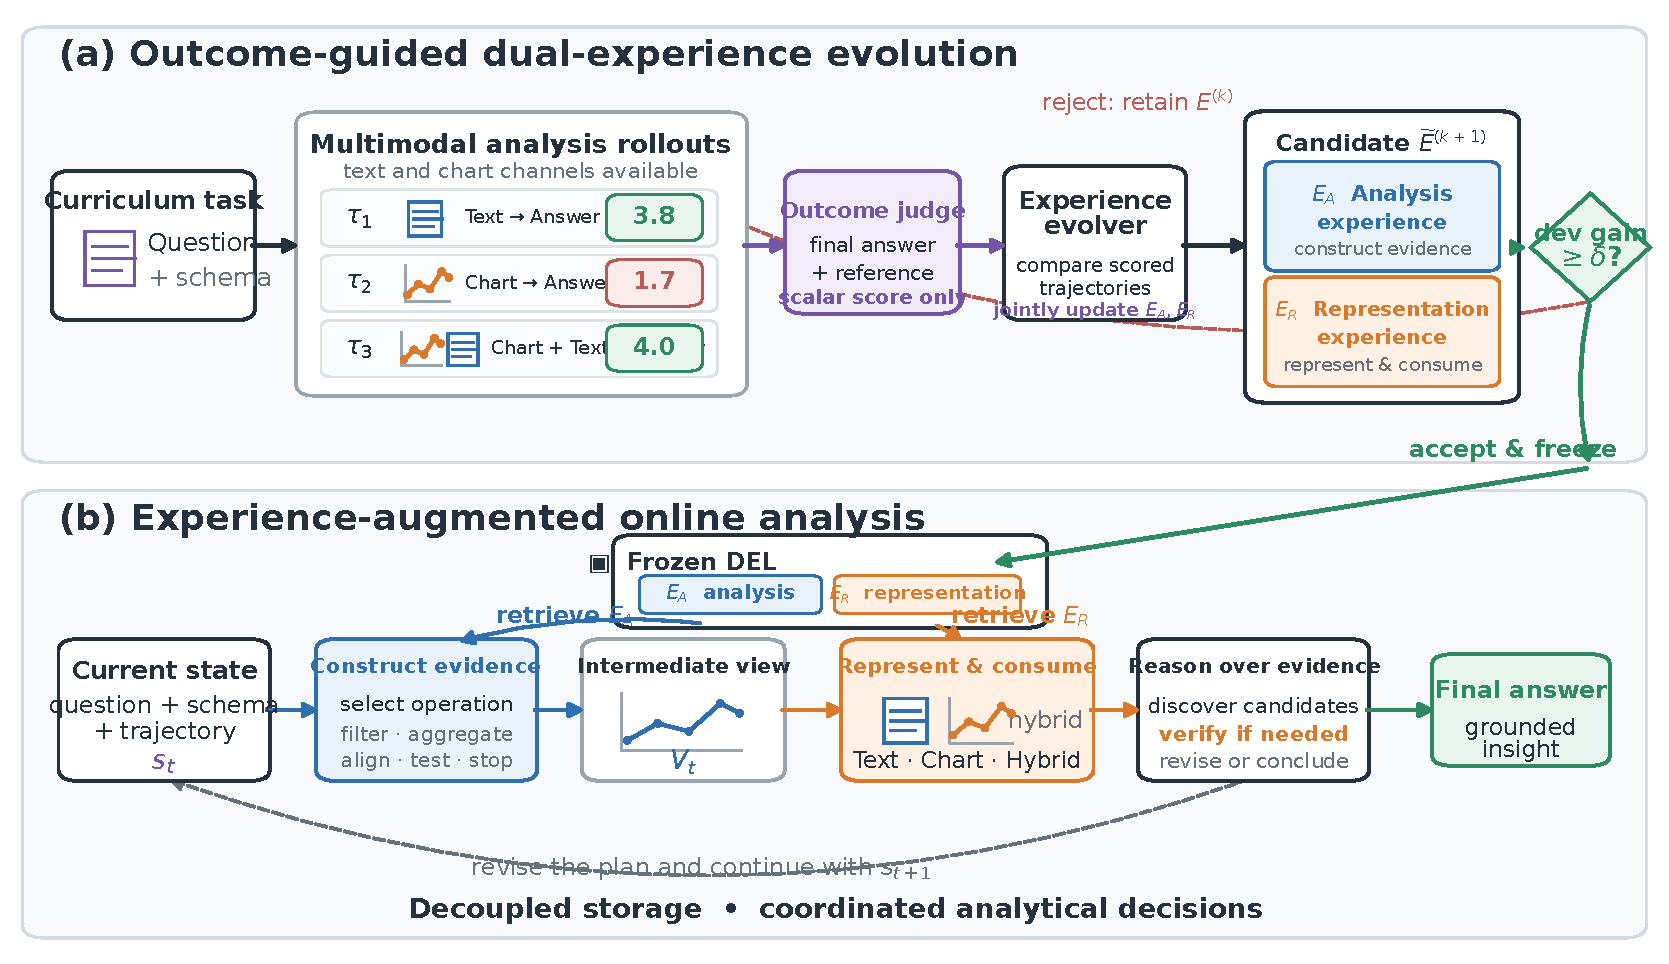
\includegraphics[width=\linewidth]{figures/care_framework_v1.pdf}
  \caption{Overview of \method{}.
    \textbf{(a)} For each curriculum task, an agent produces multiple analysis trajectories with text and chart channels available.
    An outcome judge scores only their final answers, and an experience evolver contrasts scored observable trajectories to jointly update analysis experience $E_A$ and representation experience $E_R$.
    A candidate Dual Experience Library is retained only when it improves performance on a fixed development set by at least $\delta$.
    \textbf{(b)} At inference time, the frozen library supports two coordinated decisions inside the analysis loop: $E_A$ guides which evidence to construct, while $E_R$ guides whether and how the resulting view should be consumed as text, a chart, or a hybrid representation, including numerical verification when needed.}
  \label{fig:care}
\end{figure}


\subsection{Outcome-Guided Experience Learning}
\label{sec:experience-learning}

For each curriculum task, the agent performs multiple rollouts with both text and chart channels available.
A common LLM judge scores only the final answer.
The experience evolver then compares high- and low-scoring trajectories to identify effective analytical operations, representations, and their coordination.
It jointly updates analysis experience in $E_A$ and representation experience in $E_R$.

The evolver observes the task, schema, visible trajectory, final answer, and scalar score.
It receives neither hidden reasoning nor the ground-truth insight.
This outcome-guided comparison encourages transferable strategies instead of task-specific answers.

We retain an update only when it improves performance on a fixed development set:
\begin{equation}
E^{(k+1)} =
\begin{cases}
\widetilde{E}^{(k+1)}, &
\operatorname{Score}(\widetilde{E}^{(k+1)};\mathcal{D}_{\mathrm{dev}})
-
\operatorname{Score}(E^{(k)};\mathcal{D}_{\mathrm{dev}})
\geq \delta,\\
E^{(k)}, & \text{otherwise}.
\end{cases}
\label{eq:experience-gate}
\end{equation}
\probe{} is split by flag to prevent related questions from crossing the curriculum and development sets.
The development set supports version selection only; final generalization is evaluated on held-out benchmarks.

\subsection{Online Experience Augmentation}
\label{sec:online}

After evolution, the DEL is frozen.
During online analysis, the agent first retrieves analysis experiences using the question, schema, and current trajectory state.
These experiences guide the next analytical operation and the construction of an intermediate view.
Once the view is being prepared or has been materialized, the agent retrieves representation experiences conditioned on the task objective, executed operations, and view structure.
These experiences guide whether to produce or use Text, Chart, or Hybrid representations and whether an additional numerical verification is required.
The agent then discovers candidate conclusions, verifies them when necessary, and either revises the analysis plan or produces the final answer.
Retrieved entries provide transferable strategies, applicability conditions, and failure boundaries, but do not replace contextual decision-making.
Thus, \method{} does not hard-code rules such as ``always plot trends'' in an outer controller; the agent retains responsibility for selecting the actual action from the current trajectory state.
This design allows a single model to move beyond its default modality preference and to coordinate visual discovery with symbolic verification across different stages of analysis.

\section{Experiments}
\label{sec:experiments}

The planned main evaluation spans three benchmarks with different task forms and official protocols:
long-horizon autonomous exploration, full analytical report generation, and exact-answer data-analysis question answering.
At the time of writing, \method{} results are not complete; accordingly, we specify the design and leave unfilled cells in Section~\ref{sec:main-results} explicitly marked as TBD.

\subsection{Benchmarks}
\label{sec:benchmarks}

\noindent\textbf{DDR-Bench.} Long-horizon exploratory analysis: it evaluates sustained exploration without predefined queries~\citep{liu2026ddrbench}.
We use the public, reproducible 10-K setting over a SQLite database of SEC financial disclosures for 100 companies.
The official LLM-as-checker protocol reports Message-Wise and Trajectory-Wise accuracy and their mean.

\noindent\textbf{DAComp-DA.} Analysis and report generation: it contains 100 open-ended tasks over potentially multi-table, large SQLite databases and requires a complete report with analysis, conclusions, and visualizations~\citep{lei2025dacomp}.
We report Completeness, Accuracy, Conclusiveness, Readability, Professionalism, and Visualization.
Official Overall is $60\%$ rubric correctness, $10\%$ readability, $10\%$ professionalism, and $20\%$ visualization, rather than an unweighted six-metric average.

\noindent\textbf{DSBench.} Exact-answer data analysis: it derives end-to-end tasks from real ModelOff competitions~\citep{jing2024dsbench}.
Its Data Analysis subset has 40 challenges and approximately 466 questions, with inputs that may include spreadsheets, text, and images.
We report Task-level Accuracy, competition-macro-averaged Competition-level Accuracy, and their mean.

\noindent\textbf{Isolation.} \probe{} is used for probing, experience evolution, and development gating only.
DDR-Bench, DAComp-DA, and DSBench are independent external tests held out from experience evolution.
Splits use the natural source unit---company, task, or challenge---to prevent data-source overlap.

\subsection{Experimental Setup}
\label{sec:main-exp-setup}

\noindent\textbf{Baseline.} The evaluation contains reported benchmark agents, a Baseline Agent reproduced in our common harness, and \method{}.
Baseline and \method{} use the same ReAct loop, Bash/Python/SQL tools, stdout, stderr, and chart feedback; only \method{} retrieves the frozen DEL.
Thus improvement cannot be attributed merely to access to plotting.

\noindent\textbf{LLMs.} The planned backbones are Claude Opus 5, Claude Sonnet 5, GPT-5.6 Luna, GPT-5.6 Sol, DeepSeek V4.1 Flash, and HY3.
Within each backbone, Baseline and \method{} share model version, decoding, system instructions, data access, and interaction budget.

\noindent\textbf{Experience evolution.} All DEL learning is performed on \probe{} only, using the rollout, outcome-only judge, and development-set gating procedure in Section~\ref{sec:experience-learning}.
Each backbone evolves its experience libraries independently from the same initial structure; the accepted version is frozen before evaluation on DDR-Bench, DAComp-DA, and DSBench.

Each benchmark uses its official evaluator:
DDR-Bench's GPT-5-mini checker, DAComp-DA's official rubric/GSB suite, and DSBench's answer-correctness procedure.
Methods share samples, judge prompts, and parameters within each benchmark.
Reported prior results are directly compared only when splits and protocols match.
All core comparisons are paired, with clustered bootstrap confidence intervals at the company, task, and challenge levels, respectively.

\subsection{Main Results}
\label{sec:main-results}

Cells marked ``TBD'' denote runs or official evaluations that are not yet complete; they are placeholders, not estimates.
We report each benchmark separately and do not average scores across benchmarks with incompatible scales.

\noindent\textbf{DDR-Bench.} Table~\ref{tab:ddr-matrix} reports long-horizon exploratory analysis on the reproducible 10-K setting.

\noindent\textbf{DSBench.} Table~\ref{tab:dsbench-matrix} reports exact-answer data analysis on the Data Analysis subset.

\begin{table}[t]
  \centering
  \begin{minipage}[t]{0.48\textwidth}
    \centering
    \captionof{table}{Results on \textit{DDR-Bench} benchmark.}
    \label{tab:ddr-matrix}
    \scriptsize
    \setlength{\tabcolsep}{2.5pt}
    \begin{tabular}{llccc}
      \toprule
      Method & LLM & \makecell{Msg.\\\headpct} & \makecell{Traj.\\\headpct} & \makecell{Overall\\\headpct} \\
      \midrule
      \tabpubliclyreported{5}
      ReAct & Claude Sonnet 4.5 & 77.61 & 60.58 & 69.10 \\
      ReAct & GPT-5.1 & 37.12 & 44.25 & 40.69 \\
      ReAct & GPT-5.2 & 44.89 & 41.09 & 42.99 \\
      ReAct & DeepSeek V3.2 & 60.08 & 38.15 & 49.12 \\
      ReAct & GLM-4.6 & 60.31 & 36.02 & 48.17 \\
      ReAct & Kimi K2 & 51.06 & 30.84 & 40.95 \\
      ReAct & MiniMax M2 & 44.17 & 26.88 & 35.53 \\
      \midrule
      \multirow{6}{*}{Baseline}
        % & Claude Opus 5 & TBD & TBD & TBD \\
        & Claude Sonnet 5 & 61.2 & 52.2 & 56.7 \\
        & GPT-5.6 Luna & 44.5 & 45.1 & 44.8 \\
        & GPT-5.6 Sol & 60.2 & 58.5 & 59.4 \\
        & DeepSeek V4.1 Flash & 64.2 & 59.0 & 61.6 \\
        & HY4 Preview & TBD & TBD & TBD \\
      \midrule
      \multirow{6}{*}{\method{}}
        % & Claude Opus 5 & TBD & TBD & TBD \\
        & Claude Sonnet 5 & TBD & TBD & TBD \\
        & GPT-5.6 Luna & TBD & TBD & TBD \\
        & GPT-5.6 Sol & TBD & TBD & TBD \\
        & DeepSeek V4.1 Flash & TBD & TBD & TBD \\
        & HY4 Preview & TBD & TBD & TBD \\
      \bottomrule
    \end{tabular}
  \end{minipage}\hfill
  \begin{minipage}[t]{0.48\textwidth}
    \centering
    \captionof{table}{Results on \textit{DSBench} benchmark.}
    \label{tab:dsbench-matrix}
    \scriptsize
    \setlength{\tabcolsep}{2.5pt}
    \begin{tabular}{llccc}
      \toprule
      Method & LLM & \makecell{Task\\\headpct} & \makecell{Comp.\\\headpct} & \makecell{Overall\\\headpct} \\
      \midrule
      \tabpubliclyreported{5}
      \textit{Human} & \na & 64.06 & 67.33 & 65.70 \\
      Model-only & GPT-3.5 & 20.39 & 11.85 & 16.12 \\
      Model-only & GPT-4o & 28.11 & 19.26 & 23.69 \\
      Code Inter. & GPT-3.5 & 11.16 & 8.23 & 9.70 \\
      Code Inter. & GPT-4o & 23.82 & 22.65 & 23.24 \\
      AutoGen & GPT-3.5 & 20.82 & 13.80 & 17.31 \\
      AutoGen & GPT-4o & 34.12 & 26.72 & 30.42 \\
      \midrule
      \multirow{6}{*}{Baseline}
        % & Claude Opus 5 & TBD & TBD & TBD \\
        & Claude Sonnet 5 & 88.47 & 88.42 & 88.45 \\
        & GPT-5.6 Luna & 75.11 & 73.84 & 74.47 \\
        & GPT-5.6 Sol & 89.9 & 89.4 & 89.7 \\
        & DeepSeek V4.1 Flash & TBD & TBD & TBD \\
        & HY4 Preview & 92.70 & 91.19 & 91.95 \\
      \midrule
      \multirow{6}{*}{\method{}}
        % & Claude Opus 5 & TBD & TBD & TBD \\
        & Claude Sonnet 5 & TBD & TBD & TBD \\
        & GPT-5.6 Luna & TBD & TBD & TBD \\
        & GPT-5.6 Sol & TBD & TBD & TBD \\
        & DeepSeek V4.1 Flash & TBD & TBD & TBD \\
        & HY4 Preview & TBD & TBD & TBD \\
      \bottomrule
    \end{tabular}
  \end{minipage}
\end{table}

We will report Message-Wise accuracy of \texttt{[X.X]} and Trajectory-Wise accuracy of \texttt{[Y.Y]} for \method{}, corresponding to \texttt{[$\Delta$X]} and \texttt{[$\Delta$Y]} point improvements over Baseline.
If Trajectory-Wise gains dominate, experience primarily benefits long-horizon exploration and final evidence synthesis; if both metrics rise together, \method{} improves both local insight discovery and end-to-end trajectory coverage.

\noindent\textbf{DAComp-DA.} Table~\ref{tab:dacomp-matrix} reports analysis and report generation with full analytical reports.

\begin{table}[t]
  \caption{Results on \textit{DAComp-DA} benchmark.}
  \label{tab:dacomp-matrix}
  \centering
  \scriptsize
  \setlength{\tabcolsep}{2.5pt}
  \begin{tabular}{llrrrrrrr}
    \toprule
    Method & LLM Backbone & Completeness & Accuracy & Insightfulness & Readability & Analytical Depth & Visualization & Overall \\
    \midrule
    \tabpubliclyreported{9}
    OpenHands & GPT-5 & 60.98 & 40.3 & 49.39 & 35.51 & 69.80 & 21.40 & 46.99 \\
    OpenHands & DeepSeek-V3.1 & 49.88 & 33.25 & 41.66 & 36.00 & 33.20 & 11.00 & 33.87 \\
    OpenHands & Qwen3-Coder & 33.42 & 21.21 & 25.06 & 20.00 & 13.73 & 4.80 & 24.28 \\
    DA-Agent & GPT-5 & 64.23 & 43.81 & 56.89 & 43.59 & 76.80 & 27.44 & 50.84 \\
    DA-Agent & DeepSeek-V3.1 & 48.74 & 32.97 & 42.43 & 37.25 & 35.00 & 11.45 & 34.33 \\
    DA-Agent & Qwen3-Coder & 35.12 & 20.05 & 25.53 & 19.37 & 13.42 & 5.15 & 25.13 \\
    \midrule
    \multirow{6}{*}{Baseline}
      % & Claude Opus 5 & TBD & TBD & TBD & TBD & TBD & TBD & TBD \\
      & Claude Sonnet 5 & 70.27 & 52.55 & 68.85 & 90.80 & 89.00 & 62.80 & 69.84 \\
      & GPT-5.6 Luna & 66.21 & 46.61 & 65.45 & 83.83 & 80.74 & 7.66 & 54.32 \\
      & GPT-5.6 Sol & 71.74 & 58.04 & 72.42 & 94.60 & 93.00 & 61.80 & 73.24 \\
      & DeepSeek V4.1 Flash & 83.91 & 67.80 & 81.77 & 98.0 & 94.44 & 75.72 & 82.23 \\
      & HY4 Preview & 78.55 & 60.38 & 74.39 & 96.74 & 94.78 & 66.52 & 79.40 \\
    \midrule
    \multirow{6}{*}{\method{}}
      % & Claude Opus 5 & TBD & TBD & TBD & TBD & TBD & TBD & TBD \\
      & Claude Sonnet 5 & TBD & TBD & TBD & TBD & TBD & TBD & TBD \\
      & GPT-5.6 Luna & TBD & TBD & TBD & TBD & TBD & TBD & TBD \\
      & GPT-5.6 Sol & TBD & TBD & TBD & TBD & TBD & TBD & TBD \\
      & DeepSeek V4.1 Flash & TBD & TBD & TBD & TBD & TBD & TBD & TBD \\
      % & HY3 & TBD & TBD & TBD & TBD & TBD & TBD & TBD \\
    \bottomrule
  \end{tabular}
\end{table}

We will track official Overall (from \texttt{[A]} to \texttt{[B]}) together with Completeness and Accuracy (changes \texttt{[$\Delta$C]} and \texttt{[$\Delta$A]}) to assess whether gains reflect substantive evidence and task coverage rather than surface formatting, and Visualization (\texttt{[$\Delta$V]}) to assess whether visual presentation improves.
We interpret visual representation as serving analysis only when content-correctness metrics and Visualization improve jointly.

We will report Task-level Accuracy \texttt{[X.X]} and competition-macro Competition-level Accuracy \texttt{[Y.Y]}, with Baseline-relative gains of \texttt{[$\Delta$X]} and \texttt{[$\Delta$Y]} points.
Concurrent improvements on both metrics would indicate that gains are not driven solely by competitions with many tasks; divergent changes would motivate inspection of large-competition dominance.

\noindent\textbf{Cross-benchmark synthesis.}
Across dataset--backbone pairs, we expect \method{} to outperform the matched Baseline on \texttt{[X/Y]} combinations, suggesting that jointly learning analytical operations and evidence representations transfers beyond task forms closely aligned with \probe{}---to long-horizon exploration, full report generation, and exact-answer analysis.
If effect sizes differ markedly across benchmarks, we will relate them to task openness, required analytical depth, and output modality rather than pooling raw scores.
Finer task slices, ablations, and mechanism analyses will be reported once the corresponding runs are complete; the main text will report aggregate effects with the clustered bootstrap intervals defined above.

\subsection{Planned ablations and mechanism analysis.}
The ablations compare analysis experience only, representation experience only, charts disabled, and non-evolving experiences against full \method{}.
Trajectory analysis records whether a chart triggers a new analytical operation, whether visual candidates receive numerical verification, whether charts appear only as final output, and whether unnecessary or repeated plotting occurs.
A representative case will contrast a long-text failure, correct aggregation without useful representation, and a \method{} trajectory that discovers a turning point visually and verifies its magnitude textually.
These traces explain behavior but do not substitute for benchmark outcomes.

\section{Related Work}
\label{sec:related}

\subsection{Data-analysis agents.}
LLM-driven data-analysis agents increasingly follow a plan--execute--observe--revise paradigm.
DS-Agent couples language-model reasoning with an executable analysis environment and retrieves historical cases to support data-science problem solving; Data Interpreter organizes complex tasks as dynamic directed acyclic graphs, advancing analysis through hierarchical decomposition and code execution; AIDE models machine-learning solution development as tree search in code space; DS-STAR handles heterogeneous data-analysis tasks via iterative planning and plan-sufficiency verification; and AutoKaggle and related systems adopt multi-agent division of labor for data understanding, solution planning, program development, and result review~\citep{guo2024dsagent,hong2025datainterpreter,jiang2025aide,nam2025dsstar,li2025autokaggle}.
Meanwhile, DeepAnalyze targets end-to-end coverage of data preparation, analysis, modeling, visualization, and report generation through specialized training, and InsightBench extends evaluation to open-ended, multi-step business insight generation~\citep{zhang2025deepanalyze,sahu2025insightbench}.
Although these lines of work continue to advance planning, search, collaboration, and training mechanisms, their analysis loops still rely predominantly on textual representations of structured data and on code-execution outputs as intermediate feedback.
Some systems can generate charts, but few isolate whether agents inspect self-generated charts and leverage the visual patterns they reveal to form hypotheses and steer subsequent analysis.
We focus on how visual evidence enters the intermediate reasoning loop of data-analysis agents.

\subsection{Visual modalities in data science.}
In parallel with data-analysis agents, research on visual modalities has made substantial progress in chart generation, understanding, and representational choice.
For chart generation, LIDA established a pipeline from data summaries and visualization goals to plotting code; MatPlotAgent uses rendered visual feedback to iteratively repair visualization programs; ChartMimic, AMACE, and MultiVis-Agent further improve reliability through cross-modal reconstruction, multi-agent collaboration, and iterative optimization; and ChartOptimiser shows that chart design should adapt to the analytical task at hand~\citep{dibia2023lida,yang2024matplotagent,yang2025chartmimic,namgoong2025amace,lu2026multivisagent,wang2025chartoptimiser}.
For chart understanding, UniChart, ChartLlama, and ChartBench advance chart reading and reasoning via specialized training and large-scale evaluation; DePlot, MatCha, and TinyChart improve numerical analysis through derendering, structural recovery, and programmatic reasoning; and ChartAgent and Charts-of-Thought demonstrate that visual tools combined with structured reasoning can strengthen complex chart analysis~\citep{masry2023unichart,han2023chartllama,xu2023chartbench,liu2023deplot,liu2023matcha,zhang2024tinychart,kaur2026chartagent,das2025chartsofthought}.
Building on this foundation, FRES, Format Matters, and TableDART study effectiveness differences and dynamic selection among textual, image, and chart representations, while systems such as EvidFuse construct visual evidence on demand during analysis or reporting~\citep{zhou2025fres,ho2026formatmatters,xing2026tabledart,lin2026evidfuse}.
However, existing work typically generates user-specified charts, interprets externally provided charts, or selects among pre-existing representations; it has not systematically studied data-analysis agents that start from raw structured data, jointly decide analytical operations and evidential representations, and use self-generated charts as intermediate cognitive tools for discovering patterns and advancing subsequent analysis.

\section{Conclusion}
\label{sec:conclusion}

We study how charts can serve as internal epistemic actions rather than end-of-analysis illustrations.
\probe{} shows that current LLMs can complete end-to-end analysis through self-generated charts, yet often fail to turn plotting-tool access into consistent gains, and exhibit strong model-specific biases when text and charts are both available.
Task slices indicate complementary roles: charts support trends and pattern discovery, whereas text better preserves precise, verifiable evidence.
\method{} jointly evolves analysis and representation experiences from outcome-scored trajectories, learning both what evidence to construct and how to represent and use it without hand-crafted modality rules.
Experiments on held-out benchmarks indicate that this co-evolution improves over matched baselines, supporting the view that representation choice is part of the analytical policy rather than a cosmetic output.


\bibliography{iclr2027_conference}
\bibliographystyle{iclr2027_conference}

\appendix

\section{Complete \probe{} Slice Results}
\label{app:slices}

Tasks may have multiple analytical-operation labels, while each task has one primary cognitive-operation label.
Low-$n$ rows are included for completeness and should not be interpreted as stable modality effects.

\begin{table}[h]
  \caption{Scores by analytical operation.}
  \label{tab:operation-slices}
  \centering
  \scriptsize
  \setlength{\tabcolsep}{3.5pt}
  \begin{tabular}{lrrrrr}
    \toprule
    Slice & $n$ & No-tool & Text & Chart & Free-style \\
    \midrule
    Filtering             & 109 & 0.257 & 0.752 & 0.752 & 0.755 \\
    Feature derivation    & 116 & 0.257 & 0.739 & 0.752 & 0.744 \\
    Aggregation           & 163 & 0.305 & 0.773 & 0.791 & 0.781 \\
    Normalization         &  21 & 0.143 & 0.571 & 0.512 & 0.583 \\
    Sorting               &  22 & 0.284 & 0.818 & 0.830 & 0.784 \\
    Alignment/joining     &   8 & 0.188 & 0.719 & 0.563 & 0.719 \\
    Temporal change       &  37 & 0.237 & 0.757 & 0.838 & 0.757 \\
    Distributional stats. &   1 & 1.000 & 1.000 & 1.000 & 1.000 \\
    Statistical inference &  10 & 0.200 & 0.925 & 0.900 & 0.900 \\
    Forecasting           &   3 & 0.000 & 1.000 & 1.000 & 1.000 \\
    \bottomrule
  \end{tabular}
\end{table}

\begin{table}[h]
  \caption{Scores by primary cognitive operation.}
  \label{tab:cognitive-slices}
  \centering
  \scriptsize
  \setlength{\tabcolsep}{3.5pt}
  \begin{tabular}{lrrrrr}
    \toprule
    Slice & $n$ & No-tool & Text & Chart & Free-style \\
    \midrule
    Lookup                    & 12 & 0.146 & 0.604 & 0.521 & 0.521 \\
    Scan and selection        & 24 & 0.219 & 0.958 & 0.958 & 0.958 \\
    Comparative judgment      & 69 & 0.366 & 0.801 & 0.783 & 0.808 \\
    Pattern recognition       & 54 & 0.306 & 0.769 & 0.833 & 0.764 \\
    Relational explanation    & 17 & 0.221 & 0.706 & 0.735 & 0.765 \\
    Multidimensional integration & 20 & 0.150 & 0.575 & 0.650 & 0.600 \\
    Conditional reasoning     &  4 & 0.813 & 1.000 & 0.750 & 1.000 \\
    \bottomrule
  \end{tabular}
\end{table}

\section{Items Required Before Submission}
\label{app:pending}

The final manuscript still requires: confirmation that \method{} and \probe{} do not conflict with prior names; final probe and framework artwork; a qualitative trajectory figure; pseudocode for training and online inference; completed external-benchmark and ablation results with statistical tests; judge robustness and human-agreement checks; representative experience entries and full prompts; and compute, cost, and implementation details.

\end{document}
